\makeatletter\let\ifGm@compatii\relax\makeatother
\documentclass{beamer}
\usepackage{amsfonts}
\usepackage{amsmath}
\usepackage{graphicx}
\usepackage{amssymb}
\usepackage{bm}
\usepackage{movie15}
\usepackage{color}
\usepackage{fancybox}

\mode<presentation>
{
   \usetheme{Boadilla}
}



\title[Physical properties of LiF-ThF$_4$]
{
Predictions of physical properties of LiF-ThF$_4$ \\ from molecular dynamics simulations 
}
\author[M. Levesque]{
  Maximilien Levesque, Paul Madden, Mathieu Salanne, \\ Christian Simon, Aimen Gheribi \& Patrice Chartrand}
\institute[UPMC]{
  Universit\'e Pierre et Marie Curie -- Paris -- France  \\
  University of Oxford -- UK \\
  Polytechnique Montreal -- Canada
} 
\date[June 28, 2013]{\alert{EVOL meeting - June 28, 2013}}

\begin{document}

\makeatletter
  \@ifundefined{inserttotalframenumbernew}{
    \gdef\inserttotalframenumbernew{1}
  }{}
  \gdef\inserttotalframenumber{\inserttotalframenumbernew}
\makeatother

\begin{frame}
 \titlepage
\end{frame}




\begin{frame}
  \frametitle{Outline}
  \tableofcontents
\end{frame}

\section{MD simulations}

\begin{frame}
   \frametitle{Simulation method: molecular dynamics}
   \begin{columns}
      \begin{column}{6cm}
         \begin{itemize}
            \item[$\bullet$] Newton's equation of motion solved at each time step:\\
            \begin{equation}m^i\ddot{\vec{r}}^i=\sum_{j\ne i}\vec{F}^{j\rightarrow i}=-\frac{\partial V}{\partial \vec{r}^i}\nonumber\end{equation}\\
            where $V$ is the \alert{interaction potential}
  
            \item[$\bullet$] Trajectory of particles over a few nanoseconds
            \item[$\bullet$] Determination of \alert{structural}, \alert{thermodynamic} and \alert{transport} properties
         \end{itemize}
      \end{column}
      \begin{column}{6cm}
         \begin{figure}
            \includemovie[poster,text={Loading movie}]{6cm}{6cm}{sio2na2o.mpg}
         \end{figure}
         \vspace{-0.5cm}
         \begin{center}
            {\small \it Simulation cell for SiO$_2$-Na$_2$O}
         \end{center}
      \end{column}
   \end{columns}
\end{frame}

\begin{frame}
   \frametitle{Testing the potentials: LiF-ThF$_4$}

   \begin{figure}
   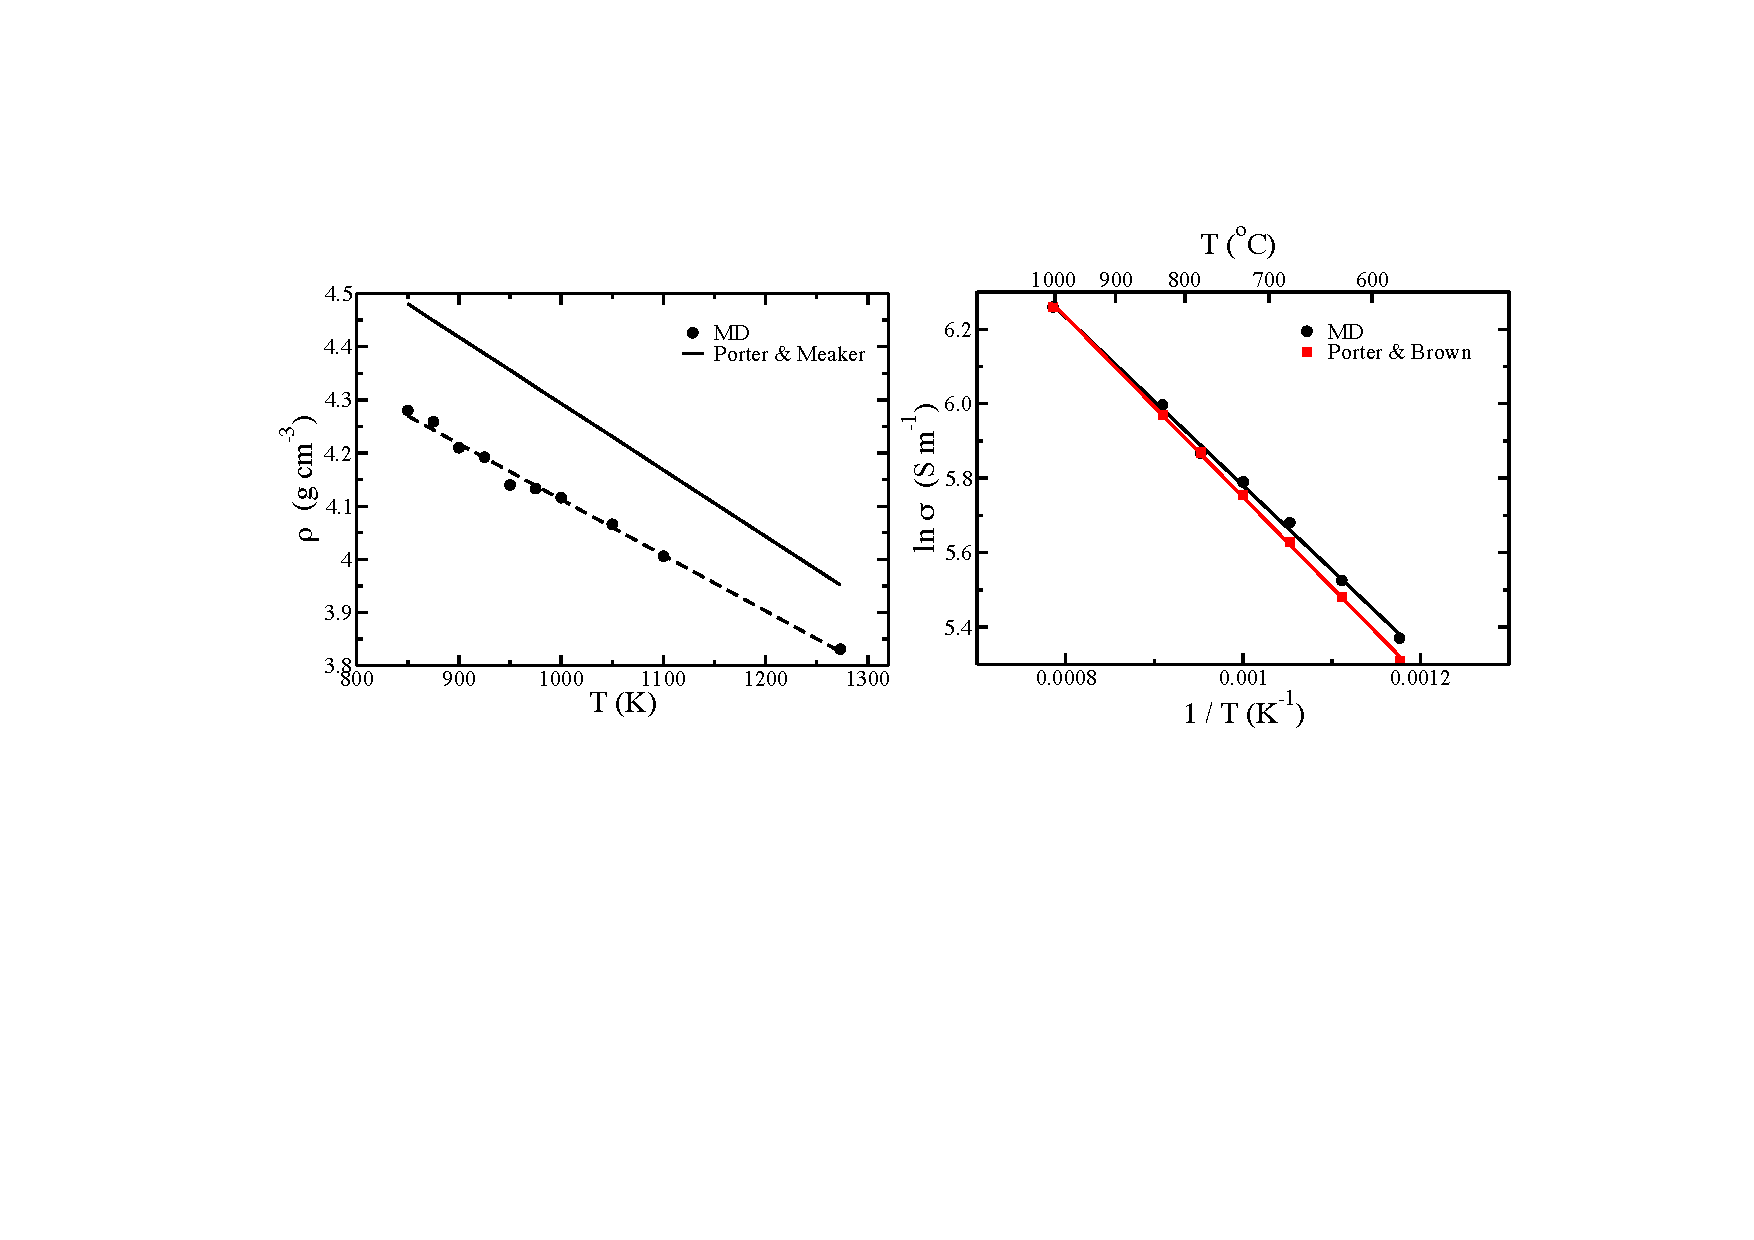
\includegraphics[width=\textwidth]{dewan-valid}
   \end{figure}

   \begin{columns}
      \begin{column}{6cm}
        \begin{itemize}
           \item[$\bullet$] Underestimation of \\ the density by $\approx$4~\%
        \end{itemize}
      \end{column}
      \begin{column}{6cm}
        \begin{itemize}
           \item[$\bullet$] Excellent accuracy \\ for the conductivity
        \end{itemize}
      \end{column}
   \end{columns}
\vspace{0.5cm}

\begin{center}
$\rightarrow$ Possible to predict all the other properties!
\end{center}

   \scriptsize{Dewan, Simon, Madden, Hobbs \& Salanne, {\it J. Nucl. Mater.}, 434, 322 (2013)}
\end{frame}



%~ 
\begin{frame}
   \frametitle{Testing the potentials: LiF-YF$_3$}
   \begin{columns}
      \begin{column}{6cm}
        \begin{equation}
            D(\alpha)=\frac{1}{6}\lim_{t\rightarrow\infty}\partial_t \left< \left| r_i(t)-r_i(0) \right|^2 \right> \nonumber
        \end{equation}
                \begin{figure}
                    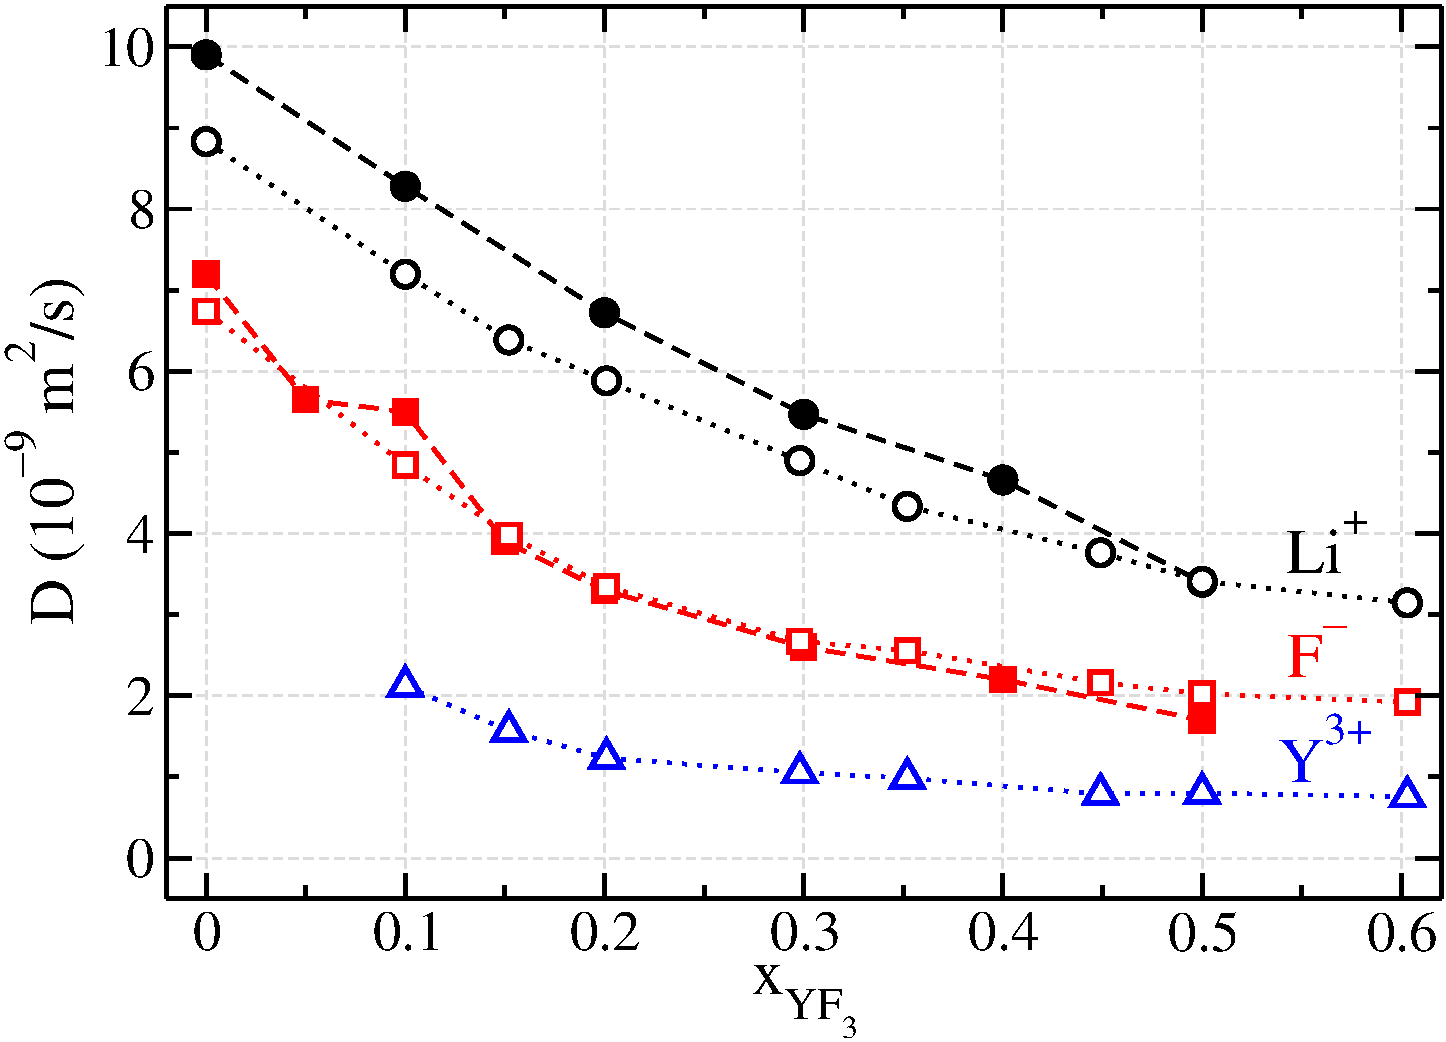
\includegraphics[width=\textwidth]{LiFYF3diffusion}
                \end{figure}
\vspace{-0.5cm}
        \begin{itemize}
           \item[$\bullet$] rel. err. for F$^-$ and Li$^+$ $<10\%$
        \end{itemize}
      \end{column}
      \begin{column}{6cm}
        \begin{itemize}
           \item[$\bullet$] Excellent accuracy \\ for the conductivity
        \end{itemize}
      \end{column}
   \end{columns}

{\scriptsize   Levesque {\it et al.}, {\it J. Chem. Phys.} {\bf 138}, 184503 (2013)}
\end{frame}
%~ 




\AtBeginSection[]
{
  \begin{frame}<beamer>
    \frametitle{Outline}
    \tableofcontents[current,currentsection]
  \end{frame}
}


\section{LiF-ThF$_4$ mixtures}

\begin{frame}
   \frametitle{Density of LiF-ThF$_4$ mixtures}
   \begin{figure}
   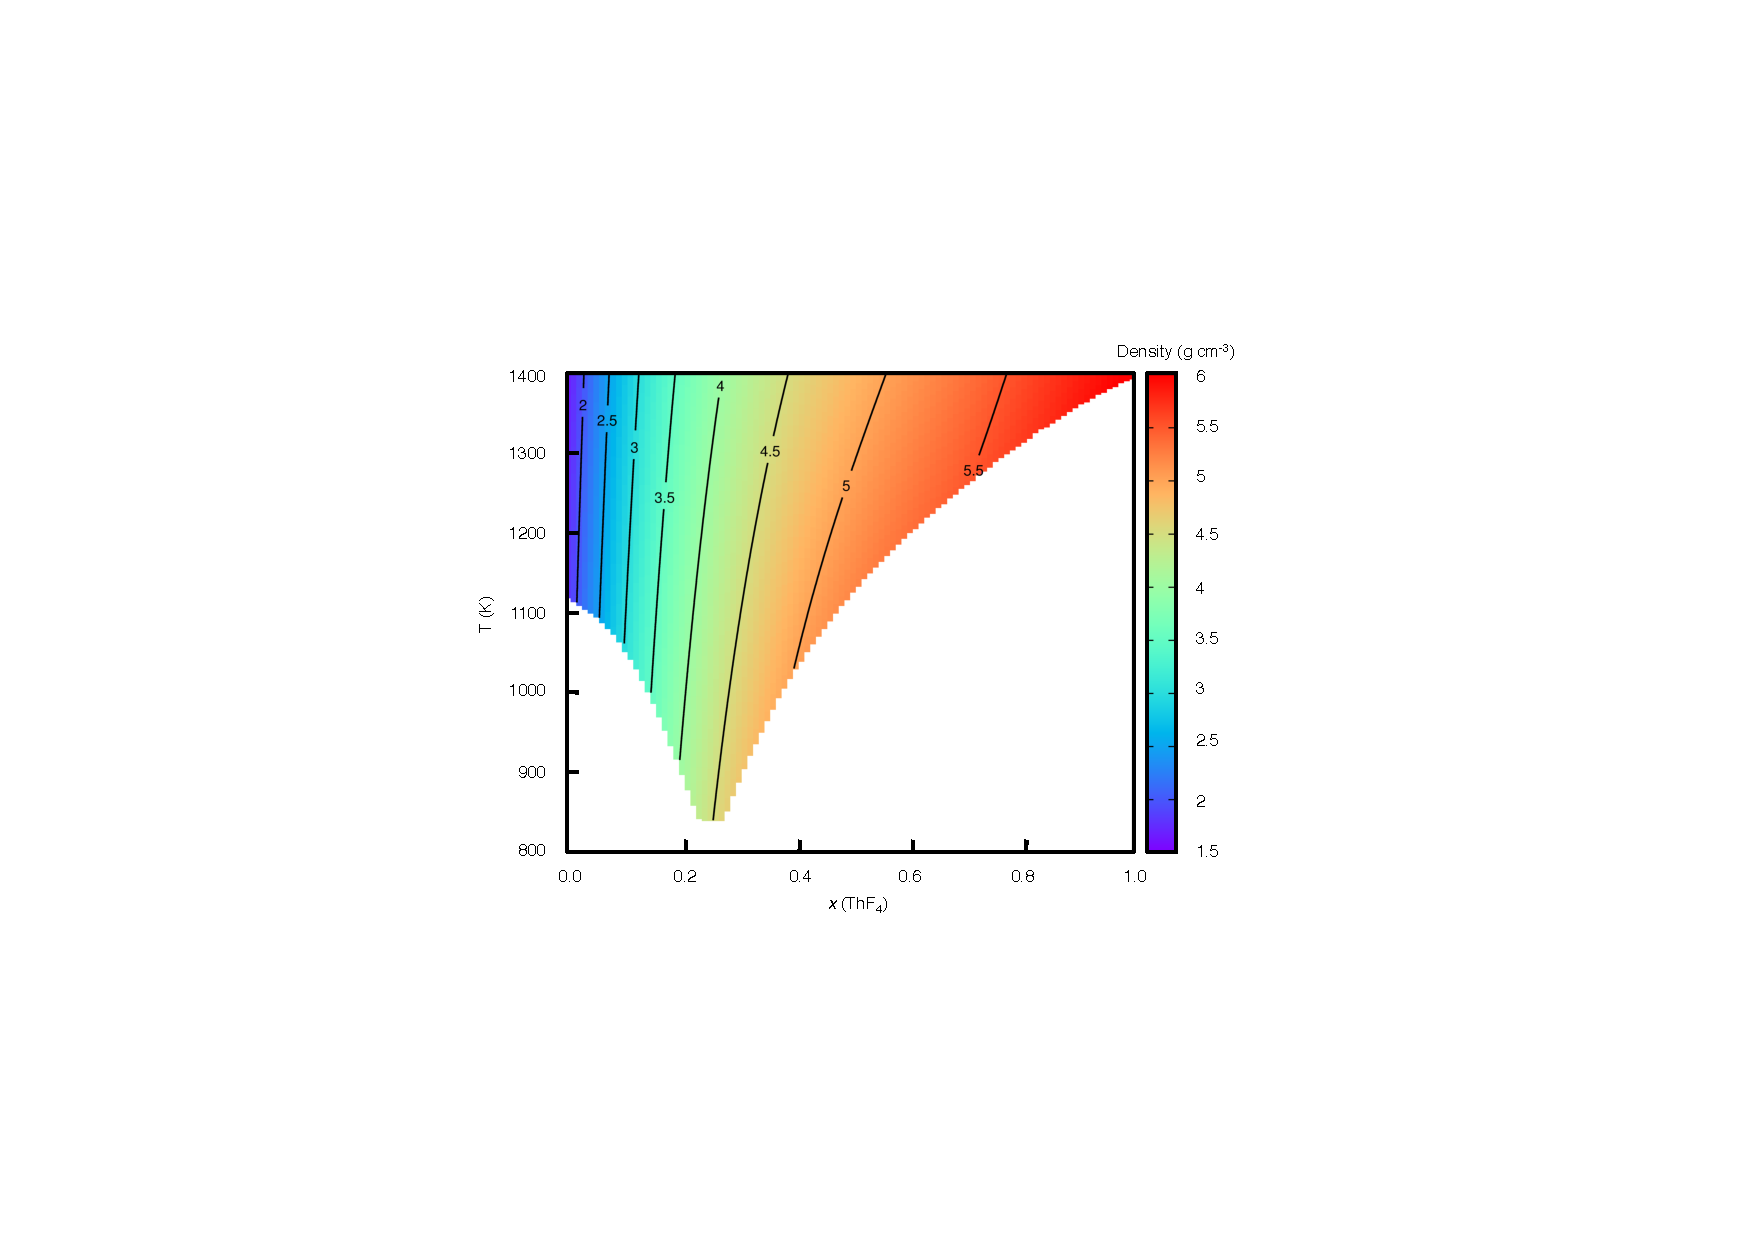
\includegraphics[width=.6\textwidth]{density}
   \end{figure}

   Calculations made for 40 different ($x_{\rm ThF_4}$, T) couples\\ and polynomial fit of the data
   
\end{frame}

\begin{frame}
   \frametitle{Viscosity of LiF-ThF$_4$ mixtures}
   \begin{figure}
   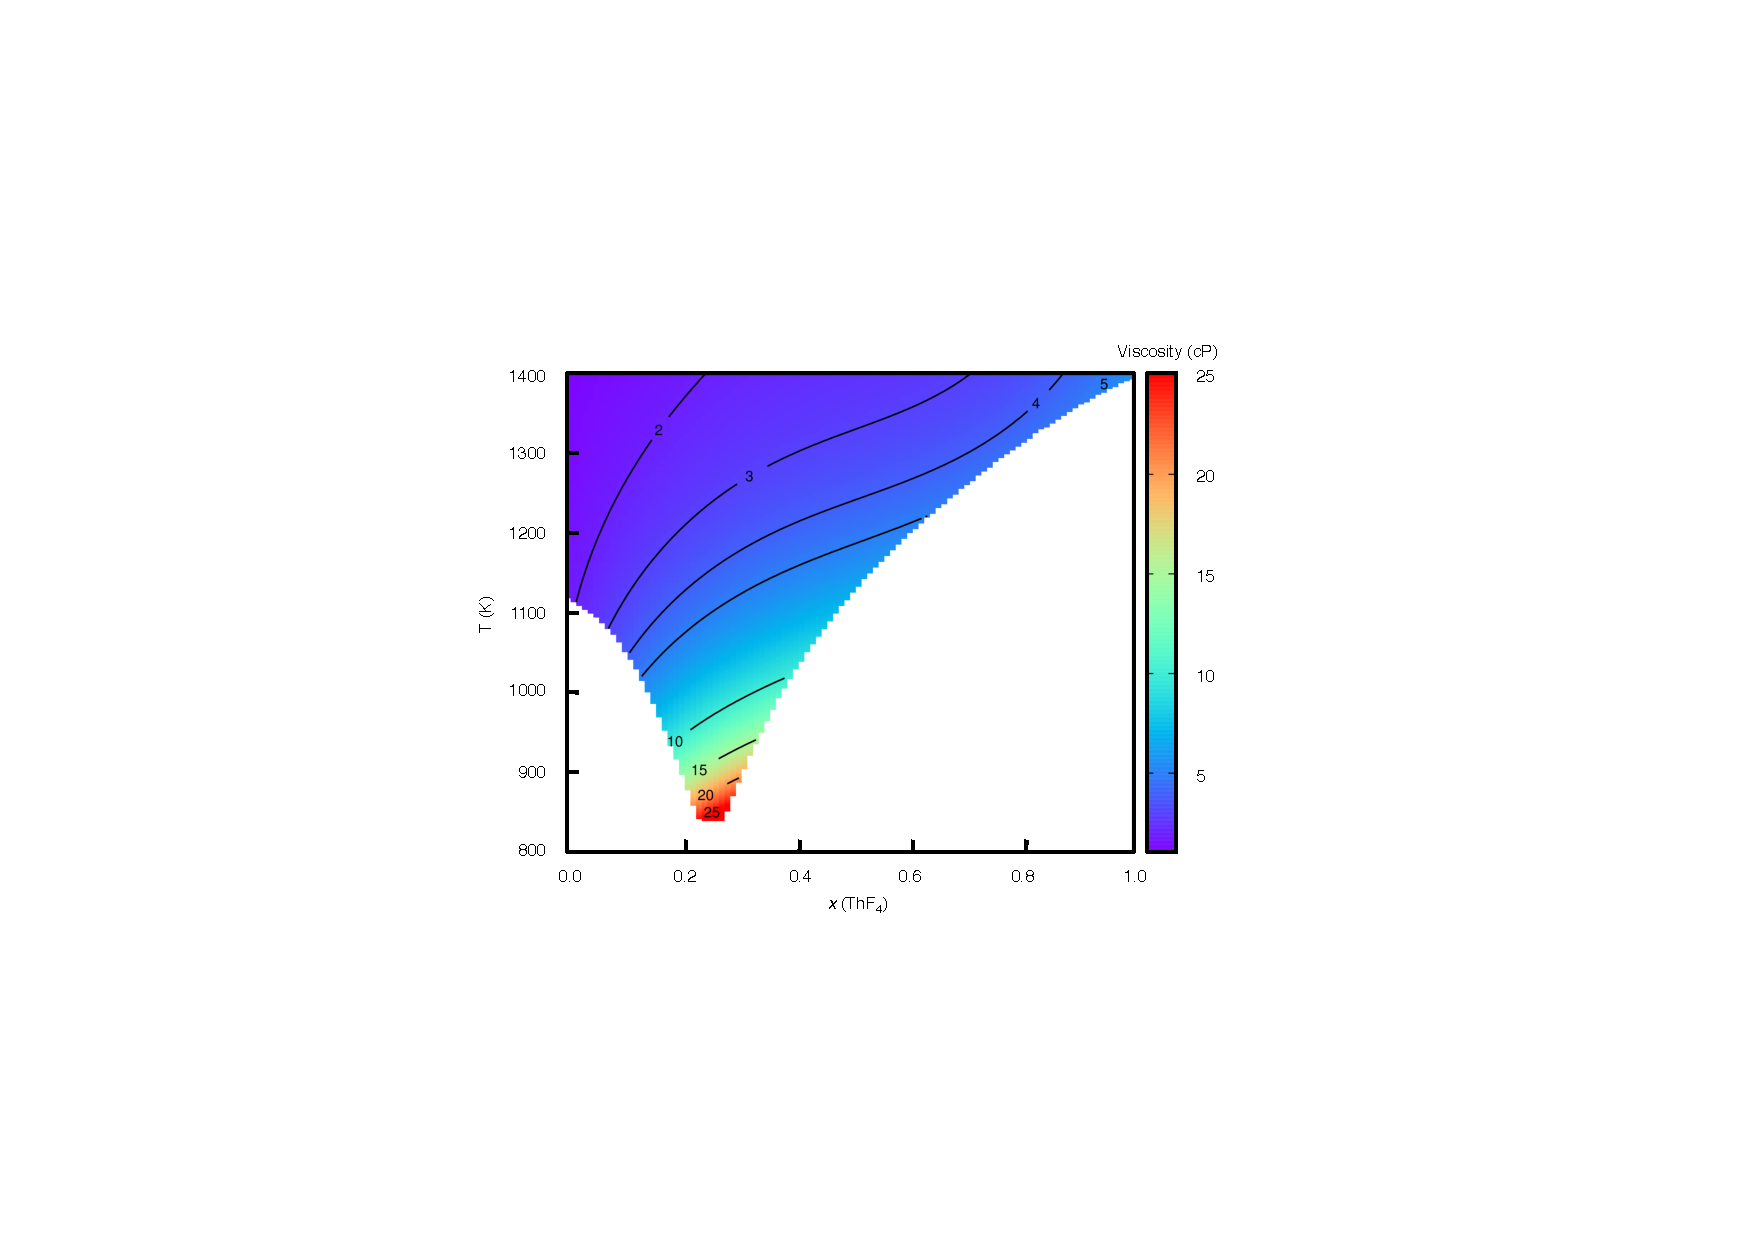
\includegraphics[width=.6\textwidth]{viscosity}
   \end{figure}

   Calculations made for 30 different ($x_{\rm ThF_4}$, T) couples\\ and polynomial fit of the data
   
\end{frame}

\begin{frame}
   \frametitle{Figures of merit}
         \[
         FOM=\frac{\eta^x}{\beta^y\rho^z C_p^t \lambda_T^u}
         \]
      \begin{itemize}
      \item[$\bullet$] $C_p$ heat capacity
      \item[$\bullet$] $\rho$ density
      \item[$\bullet$] $\eta$ viscosity
      \item[$\bullet$]  $\beta$ thermal expansion
      \item[$\bullet$] $\lambda_T$ thermal conductivity
   \end{itemize}

\vspace{1cm}
{\scriptsize  C. Bonilla, {\it Nuclear Engineering Handbook}, 9-90 (1958)}
\end{frame}

\begin{frame}
   \frametitle{Forced convection, turbulent r\'egime}
   \begin{figure}
   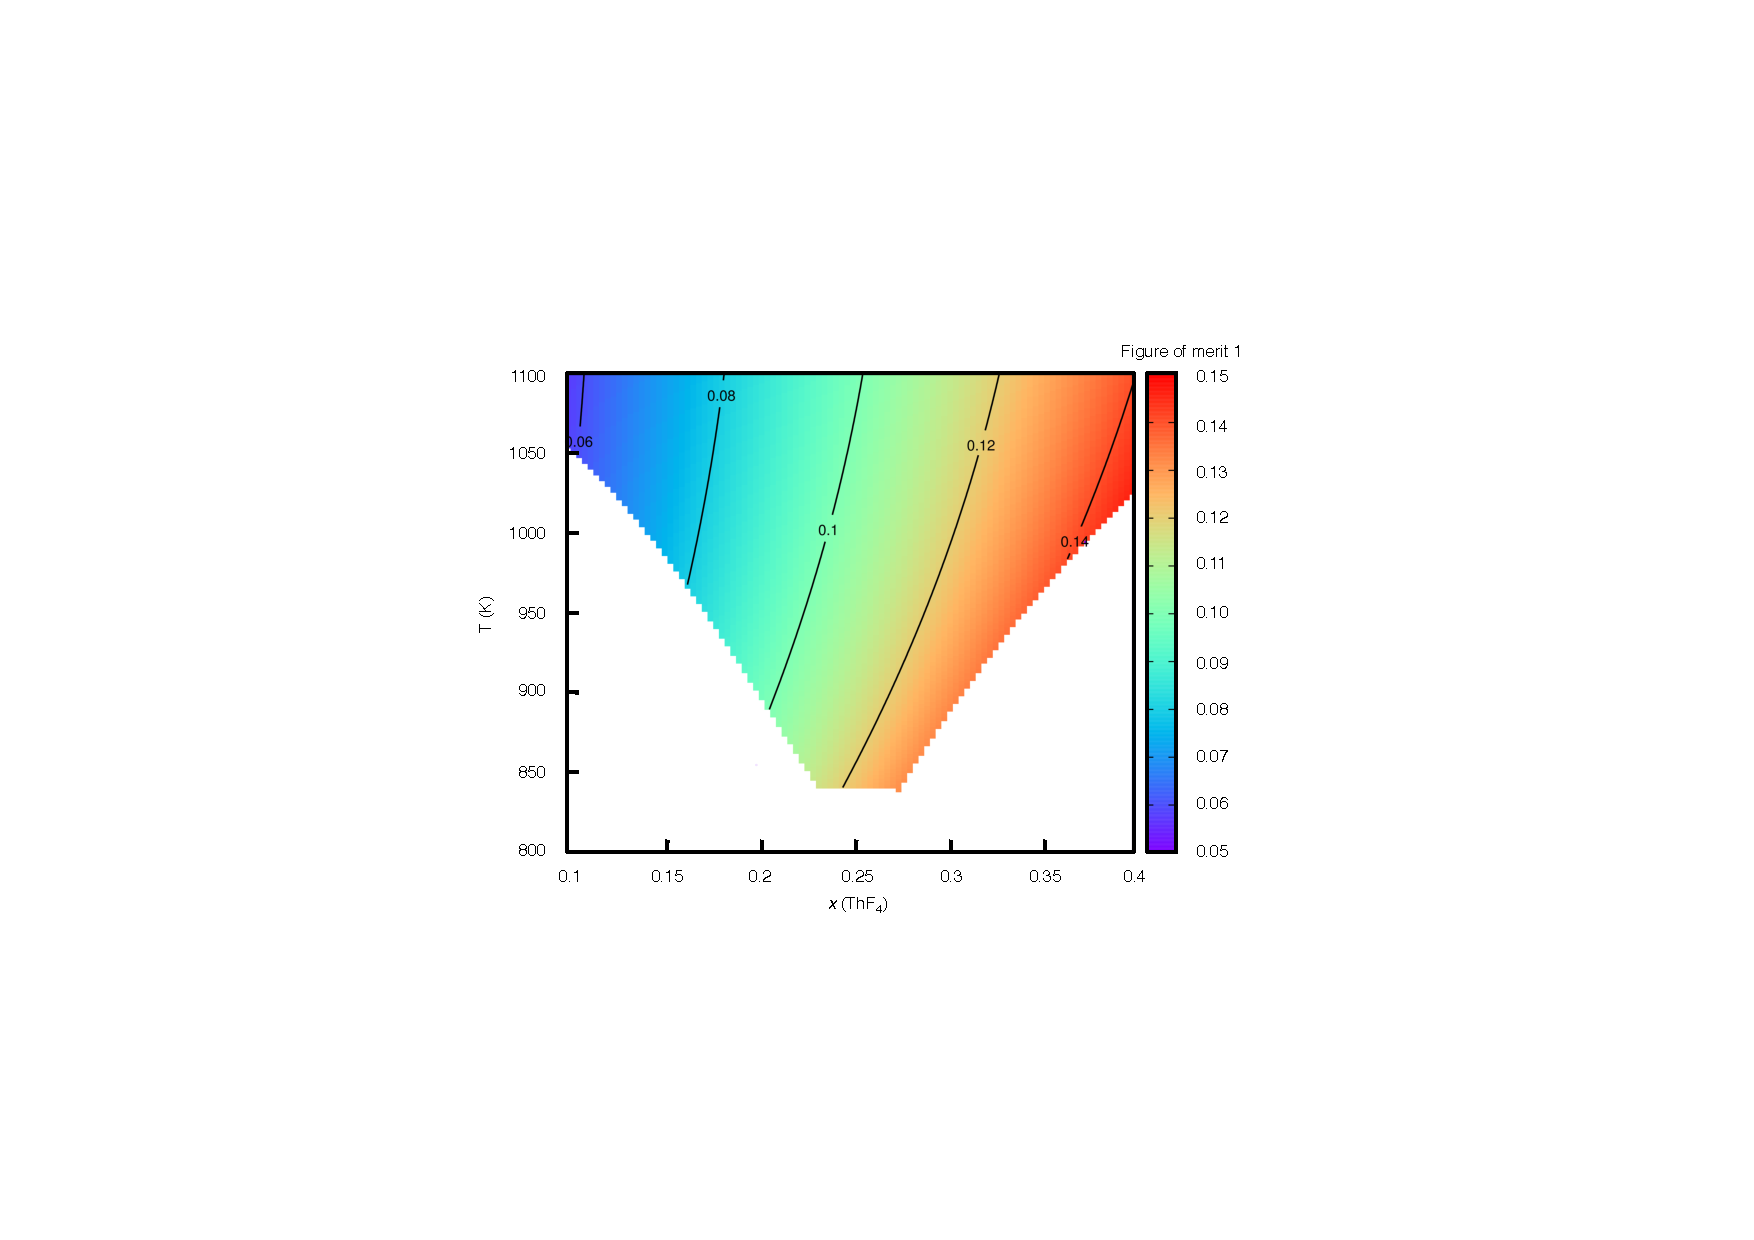
\includegraphics[width=.6\textwidth]{merit1}
   \end{figure}

  Other salts at 873~K:
    \begin{columns}
      \begin{column}{6cm}
        \begin{itemize}
           \item[$\bullet$] FLiNaK: 0.063
        \end{itemize}
      \end{column}
      \begin{column}{6cm}
        \begin{itemize}
           \item[$\bullet$] NaF-ZrF$_4$ eutectic: 0.126
        \end{itemize}
      \end{column}
   \end{columns}
   
\end{frame}

\begin{frame}
   \frametitle{Natural convection, turbulent r\'egime}
   \begin{figure}
   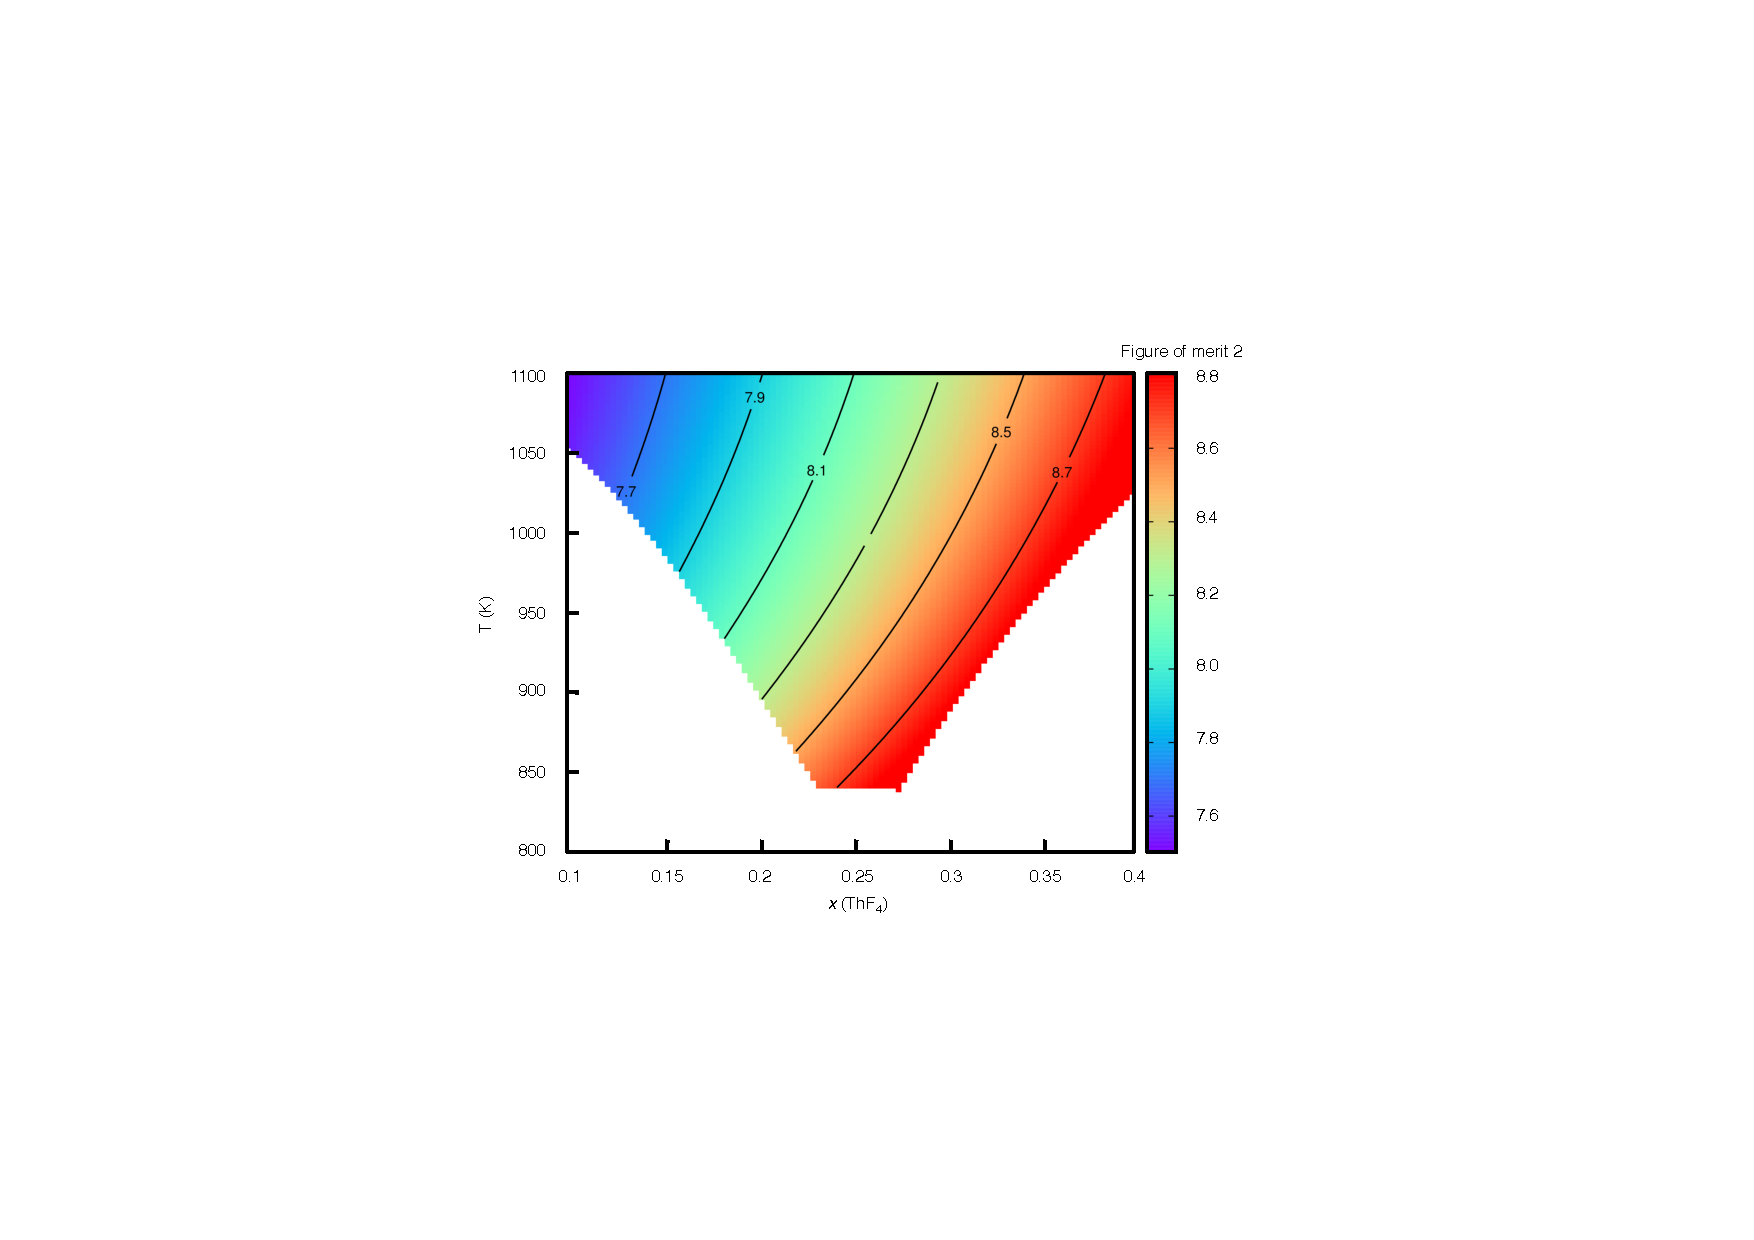
\includegraphics[width=.6\textwidth]{merit2}
   \end{figure}

  Other salts at 873~K:
    \begin{columns}
      \begin{column}{6cm}
        \begin{itemize}
           \item[$\bullet$] FLiNaK: 8.01 
        \end{itemize}
      \end{column}
      \begin{column}{6cm}
        \begin{itemize}
           \item[$\bullet$] NaF-ZrF$_4$ eutectic: 8.98
        \end{itemize}
      \end{column}
   \end{columns}
   
\end{frame}

\begin{frame}
   \frametitle{Natural convection, laminar r\'egime}
   \begin{figure}
   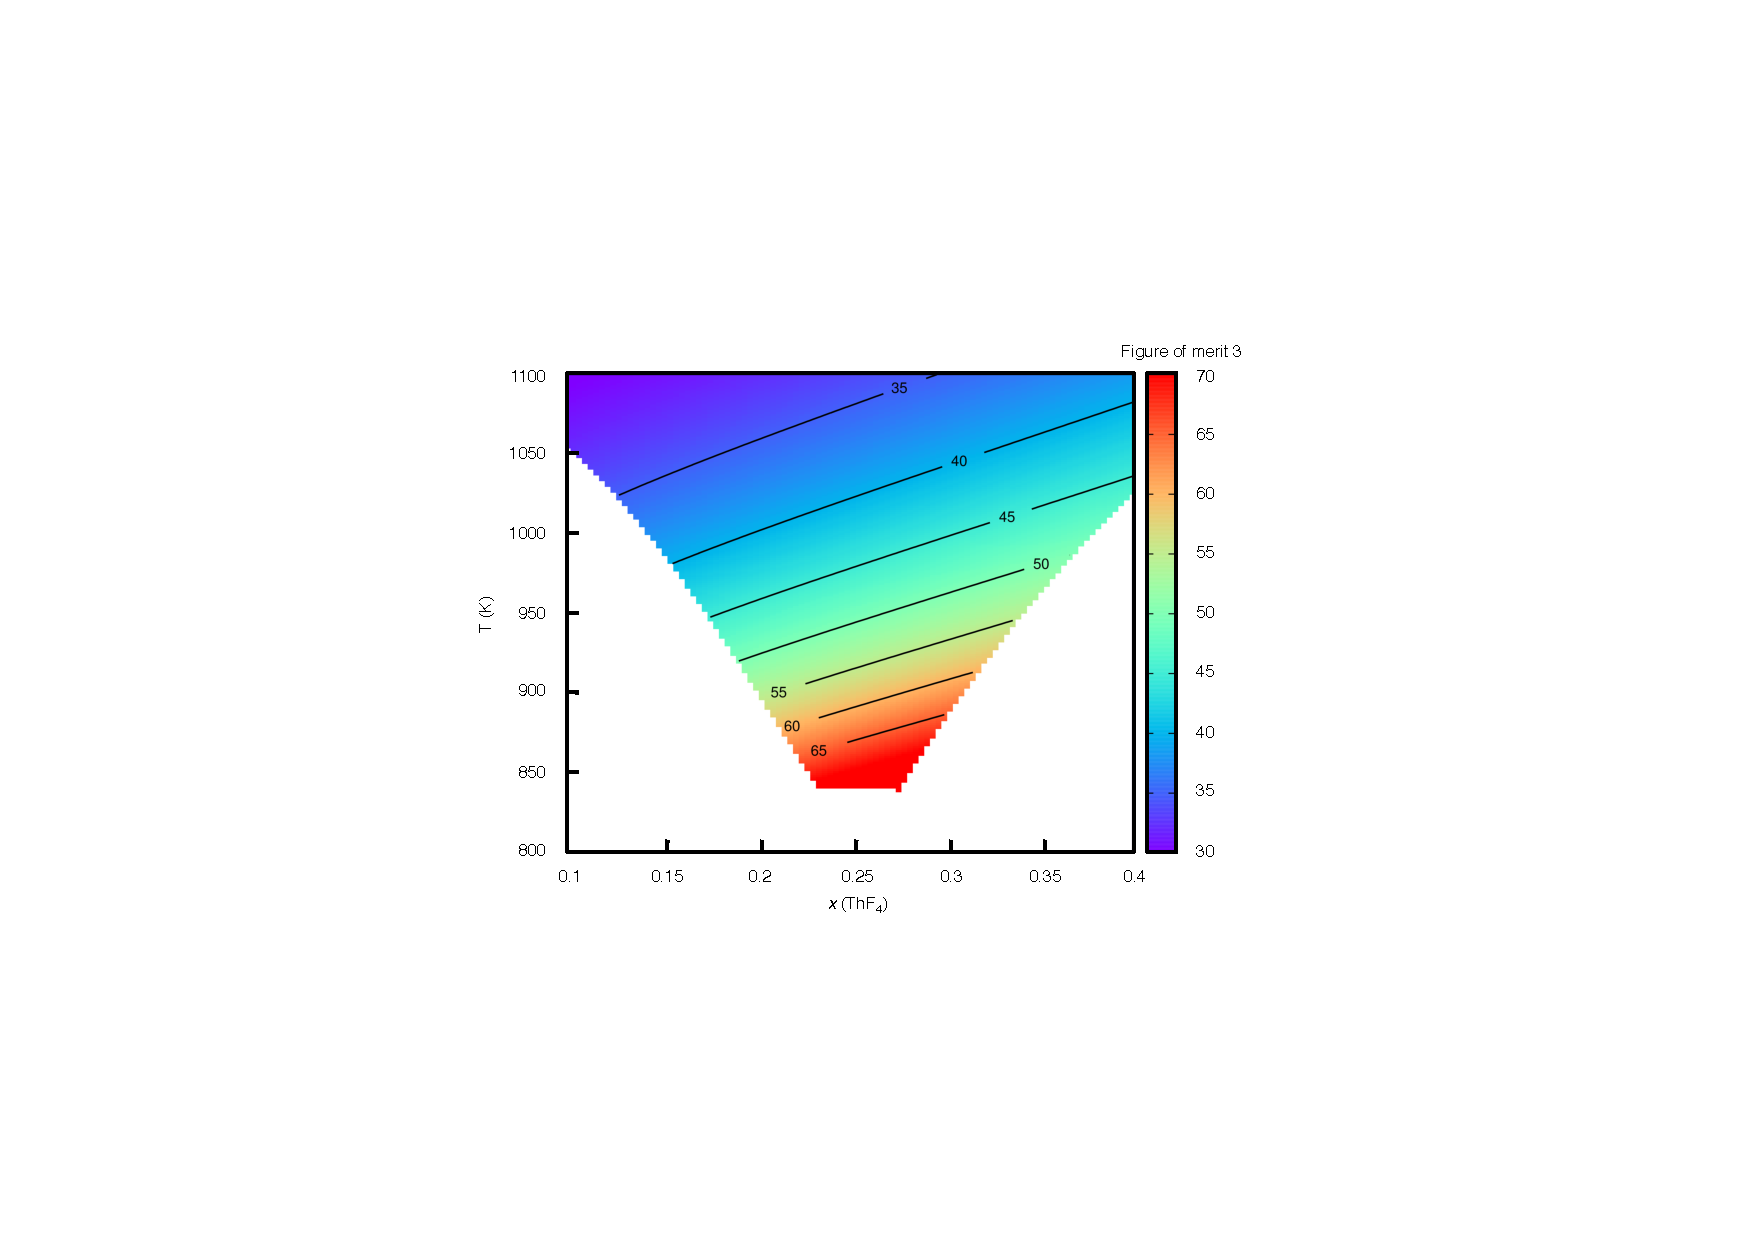
\includegraphics[width=.6\textwidth]{merit3}
   \end{figure}

  Other salts at 873~K:
    \begin{columns}
      \begin{column}{6cm}
        \begin{itemize}
           \item[$\bullet$] FLiNaK: 31.45
        \end{itemize}
      \end{column}
      \begin{column}{6cm}
        \begin{itemize}
           \item[$\bullet$] NaF-ZrF$_4$ eutectic: 41.74
        \end{itemize}
      \end{column}
   \end{columns}
   
\end{frame}

\section{Activity coefficients}

\section{Conclusion \& Perspectives}

\begin{frame}
   \frametitle{Conclusion}
   \begin{itemize}
      \item[$\bullet$] Interaction potentials including many-body polarization effects for a series of molten fluorides
      \item[$\bullet$] Parameterization from first-principles calculations
      \item[$\bullet$] Prediction of transport properties of LiF-ThF$_4$ across the whole range of coompositions/temperatures
      \item[$\bullet$] \alert{Activity coefficients in molten fluorides} 
   \end{itemize}
\end{frame}

\appendix
\makeatletter
  \immediate\write\@mainaux{\string\gdef\string\inserttotalframenumbernew{\insertframenumber}}
\makeatother





\end{document}
